\documentclass[11pt]{article}

\usepackage{amsmath,amsthm,amsfonts,amssymb,amsxtra}
\usepackage{pgf,tikz}
\usepackage{pgfplots}
\pgfplotsset{compat=1.11}
\usepackage{mathrsfs}
\renewcommand{\theenumi}{(\alph{enumi})} 
\renewcommand{\labelenumi}{\theenumi}

\pagestyle{empty}
\setlength{\textwidth}{7in}
\setlength{\oddsidemargin}{-0.5in}
\setlength{\topmargin}{-1.0in}
\setlength{\textheight}{9.5in}

\theoremstyle{definition}
\newtheorem{problem}{Problem}
\theoremstyle{theorem}
\newtheorem*{theorem}{Theorem}

\begin{document}

\noindent{\large\bf MATH 300}\hfill{\large\bf Test \#2}\hfill{\large\bf Fall 2018}\hfill{\large\bf Page 1/11}\hrule

\bigskip
\begin{center}
  \begin{tabular}{|ll|}
    \hline & \cr
    {\bf Name: } & \makebox[12cm]{\hrulefill}\cr & \cr
    {\bf VIP ID:} & \makebox[12cm]{\hrulefill}\cr & \cr
    \hline
  \end{tabular}
\end{center}
\begin{itemize}
\item Write your name and VIP ID in the space provided above.
\item The test has eleven (11) pages, including this one.
\item Credit for each problem is given at the right of each problem number.
\item Make sure to \textbf{box} your proofs, to differentiate them from your exploration and planning.  I will only grade
  for boxed content on each submission.
\item Make sure to provide only \textbf{direct proofs}.  I will test your skill with other techniques in a different test.
\item No books, notes or calculators are allowed.
\end{itemize}
\hrule

\begin{center}
  \begin{tabular}{|c|c|c||c|c|c|}
    \hline
    &&&&& \\
    {\large\bf Page} & {\large\bf Max} & {\large\bf Points} & {\large\bf Page} & {\large\bf Max} & {\large\bf Points} \\
    &&&&& \\ \hline
    &&&&& \\
    {\Large 2} & {\Large 10} &  & {\Large 7} & {\Large 10} & \\
    &&&&& \\ \hline
    &&&&& \\
    {\Large 3} & {\Large 10} &  & {\Large 8} & {\Large 10} & \\
    &&&&& \\ \hline
    &&&&& \\
    {\Large 4} & {\Large 10} &  & {\Large 9} & {\Large 10} & \\
    &&&&& \\ \hline
    &&&&& \\
    {\Large 5} & {\Large 10} &  & {\Large 10} & {\Large 10} & \\
    &&&&& \\ \hline
    &&&&& \\
    {\Large 6} & {\Large 10} &  & {\Large 11} & {\Large 10} & \\
    &&&&& \\ \hline \hline
    &&&&& \\
    {\large\bf Total} & & & & & \\
    &&&&& \\ \hline
  \end{tabular}
\end{center}
\newpage

%%%%%%%%%%%%%%%%%%%%%%%%%%%%%%%%%%%%%%%%%%%%%%%%%%%%%%%%%%%%%%%%%%%%% Page 2
\noindent{\large\bf MATH 300}\hfill{\large\bf Test \#2}\hfill{\large\bf Fall 2018}\hfill{\large\bf Page 2/11}\hrule

\bigskip
\begin{problem}[10 pts]
  Prove the following result:
  \vspace{-0.75cm}
  \begin{quotation}
    \begin{theorem}
      If $x$ and $y$ are odd integers, then $xy$ is an odd integer.
    \end{theorem}
  \end{quotation}
\end{problem}
\newpage

%%%%%%%%%%%%%%%%%%%%%%%%%%%%%%%%%%%%%%%%%%%%%%%%%%%%%%%%%%%%%%%%%%%%% Page 3
\noindent{\large\bf MATH 300}\hfill{\large\bf Test \#2}\hfill{\large\bf Fall 2018}\hfill{\large\bf Page 3/11}\hrule

\bigskip
\begin{problem}[10 pts]
  Prove the following result:
  \vspace{-0.75cm}
  \begin{quotation}
    \begin{theorem}
      If $b$ and $c$ are odd integers and $a$ is any integer, then $ab+ac$ is an even integer.
    \end{theorem}
  \end{quotation}
\end{problem}
\newpage

%%%%%%%%%%%%%%%%%%%%%%%%%%%%%%%%%%%%%%%%%%%%%%%%%%%%%%%%%%%%%%%%%%%%% Page 4
\noindent{\large\bf MATH 300}\hfill{\large\bf Test \#2}\hfill{\large\bf Fall 2018}\hfill{\large\bf Page 4/11}\hrule

\bigskip
\begin{problem}[10 pts]
  Prove the following result:
  \vspace{-0.75cm}
  \begin{quotation}
    \begin{theorem}
      If two integers have opposite parity, then their sum is odd.
    \end{theorem}
  \end{quotation}
\end{problem}
\newpage

%%%%%%%%%%%%%%%%%%%%%%%%%%%%%%%%%%%%%%%%%%%%%%%%%%%%%%%%%%%%%%%%%%%%% Page 5
\noindent{\large\bf MATH 300}\hfill{\large\bf Test \#2}\hfill{\large\bf Fall 2018}\hfill{\large\bf Page 5/11}\hrule

\bigskip
\begin{problem}[10 pts]
  Prove the following result:
  \vspace{-0.75cm}
  \begin{quotation}
    \begin{theorem}
      Let $x$ and $y$ be positive numbers.  If $x \leq y$, then $\sqrt{x} \leq \sqrt{y}$.
    \end{theorem}
  \end{quotation}
\end{problem}
\newpage

%%%%%%%%%%%%%%%%%%%%%%%%%%%%%%%%%%%%%%%%%%%%%%%%%%%%%%%%%%%%%%%%%%%%% Page 6
\noindent{\large\bf MATH 300}\hfill{\large\bf Test \#2}\hfill{\large\bf Fall 2018}\hfill{\large\bf Page 6/11}\hrule

\bigskip
\begin{problem}[10 pts--5 pts each part]
  Prove the following result:
  \vspace{-0.75cm}
  \begin{quotation}
    \begin{theorem}
      If the equation $ax^2+bx+c=0$ has two different real-valued solutions, then
      \begin{enumerate}
      \item The sum of the two solutions is equal to $-b/a$.
      \item The product of the two solutions is equal to $c/a$.
      \end{enumerate}
    \end{theorem}
  \end{quotation}
\end{problem}
\newpage

%%%%%%%%%%%%%%%%%%%%%%%%%%%%%%%%%%%%%%%%%%%%%%%%%%%%%%%%%%%%%%%%%%%%% Page 7
\noindent{\large\bf MATH 300}\hfill{\large\bf Test \#2}\hfill{\large\bf Fall 2018}\hfill{\large\bf Page 7/11}\hrule

\bigskip
\begin{problem}[10 pts--1,1,4,4]
  The first two steps will help you with the Theorem in this page.
  \begin{enumerate}
  \item Apply polynomial division to compute $\dfrac{x^2-1}{x-1}$.  Or if you prefer, simply \emph{factor} $x^2-1$.
    \vspace{2cm}
  \item Apply polynomial division to compute $\dfrac{x^3+1}{x+1}$.  Or if you prefer, simply \emph{factor} $x^3+1$.
    \vspace{3cm}
  \item Prove the following result:
    \vspace{-0.75cm}
    \begin{quotation}
      \begin{theorem}
        For each integer $a$, if 4 divides $a+1$, then 4 also divides $a^3+1$.
      \end{theorem}
    \end{quotation}
    \vspace{3cm}
  \item Prove the following result:
    \vspace{-0.75cm}
    \begin{quotation}
      \begin{theorem}
        For each integer $a$, if 5 divides $a+2$, then 5 also divides $2a^3+7a^2+6a$.
      \end{theorem}
    \end{quotation}
  \end{enumerate}
\end{problem}
\newpage

%%%%%%%%%%%%%%%%%%%%%%%%%%%%%%%%%%%%%%%%%%%%%%%%%%%%%%%%%%%%%%%%%%%%% Page 8
\noindent{\large\bf MATH 300}\hfill{\large\bf Test \#2}\hfill{\large\bf Fall 2018}\hfill{\large\bf Page 8/11}\hrule

\bigskip
\begin{problem}[10 pts]
  Prove the following result:
  \vspace{-0.75cm}
  \begin{quotation}
    \begin{theorem}
      If the \textbf{greatest common divisor} of two natural numbers $a, b$ is greater than 1, then $b \mid a$ or $b$ is
      not prime.
    \end{theorem}
  \end{quotation}
\end{problem}
\newpage

%%%%%%%%%%%%%%%%%%%%%%%%%%%%%%%%%%%%%%%%%%%%%%%%%%%%%%%%%%%%%%%%%%%%% Page 9
\noindent{\large\bf MATH 300}\hfill{\large\bf Test \#2}\hfill{\large\bf Fall 2018}\hfill{\large\bf Page 9/11}\hrule

\bigskip
\begin{problem}[10 pts]
  Prove the following result:
  \vspace{-0.75cm}
  \begin{quotation}
    \begin{theorem}
      If $x \in \mathbb{R}$ and $0 < x < 3/2$, then $8x(3-2x) \leq 9$.
    \end{theorem}
  \end{quotation}
\end{problem}
\newpage

%%%%%%%%%%%%%%%%%%%%%%%%%%%%%%%%%%%%%%%%%%%%%%%%%%%%%%%%%%%%%%%%%%%%% Page 10
\noindent{\large\bf MATH 300}\hfill{\large\bf Test \#2}\hfill{\large\bf Fall 2018}\hfill{\large\bf Page 10/11}\hrule

\bigskip
\begin{problem}[10 pts--2.5 pts each part]
  The following steps will help you with the Theorem in Problem \ref{p:Maria}
  \begin{enumerate}
  \item Sketch the region $A$ of the plane given by the inequality $y>2$.  Write $A$ in set-builder notation.
    \begin{equation*} A = \framebox[8cm]{\textcolor{white}{$\Huge\int \dfrac{x}{x^2}$}} \end{equation*}
  \item Sketch the region $B$ of the plane given by the inequality $x<-4$.  Write $B$ in set-builder notation.
    $B$.
    \begin{equation*} B =  \framebox[8cm]{\textcolor{white}{$\Huge\int \dfrac{x}{x^2}$}} \end{equation*}
  \item Write down the formula for the distance $d$ from any point $(x,y)$ to the point $(1,-2)$.  Draw the curves with
    implicit equation $(x-1)^2 + (y+2)^2 = R^2$, for $R=2,3,4,5,6,7$.
    \begin{equation*} d =  \framebox[8cm]{\textcolor{white}{$\Huge\int \dfrac{x}{x^2}$}} \end{equation*}
  \item How far is the point $(1,-2)$ from the vertical line $x=-4$?  How far is the point $(1,-2)$ from the horizontal
    line $y=2$?  What is the closest point from $A \cap B$ to the point $(1,-2)$?
  \end{enumerate}
  \vspace{4.9cm}
  \hrule
  \begin{center}
    \begin{tikzpicture}[scale=1.6]
      \begin{axis}[
        xmin=-8,xmax=8,
        ymin=-6,ymax=6,
        grid=both,
        grid style={line width=.1pt, draw=gray!10},
        major grid style={line width=.2pt,draw=gray!50},
        axis lines=middle,
        minor tick num=5,
        axis line style={latex-latex},
        ticklabel style={font=\tiny},
        xlabel style={at={(ticklabel* cs:1)},anchor=north west},
        ylabel style={at={(ticklabel* cs:1)},anchor=south west},
        ]
      \end{axis}
    \end{tikzpicture}
  \end{center}
\end{problem}
\newpage

%%%%%%%%%%%%%%%%%%%%%%%%%%%%%%%%%%%%%%%%%%%%%%%%%%%%%%%%%%%%%%%%%%%%% Page 11
\noindent{\large\bf MATH 300}\hfill{\large\bf Test \#2}\hfill{\large\bf Fall 2018}\hfill{\large\bf Page 11/11}\hrule

\bigskip
\begin{problem}[10 pts]\label{p:Maria} 
  Prove the following result:
  \vspace{-0.75cm}
  \begin{quotation}
    \begin{theorem}
      If $x<-4$ and $y>2$, then the distance from $(x,y)$ to $(1,-2)$ is at least 6.
    \end{theorem}
  \end{quotation}
\end{problem}
\end{document}



%%% Local Variables:
%%% mode: latex
%%% TeX-master: t
%%% End:
